\section{Ausgangslage}

Das Bundesamt für Informatik und Telekommunikation verfolgt mit dem Swiss Government Cloud (SGC) Vorhaben die Transformation der Cloud-Infrastruktur der Bundesverwaltung. Vision ist es einen auf die Bedürfnisse des Bundes zugeschnittene hybride Multi-Cloud Infrastruktur aufzubauen.

\begin{figure}[H]
    \begin{center}
        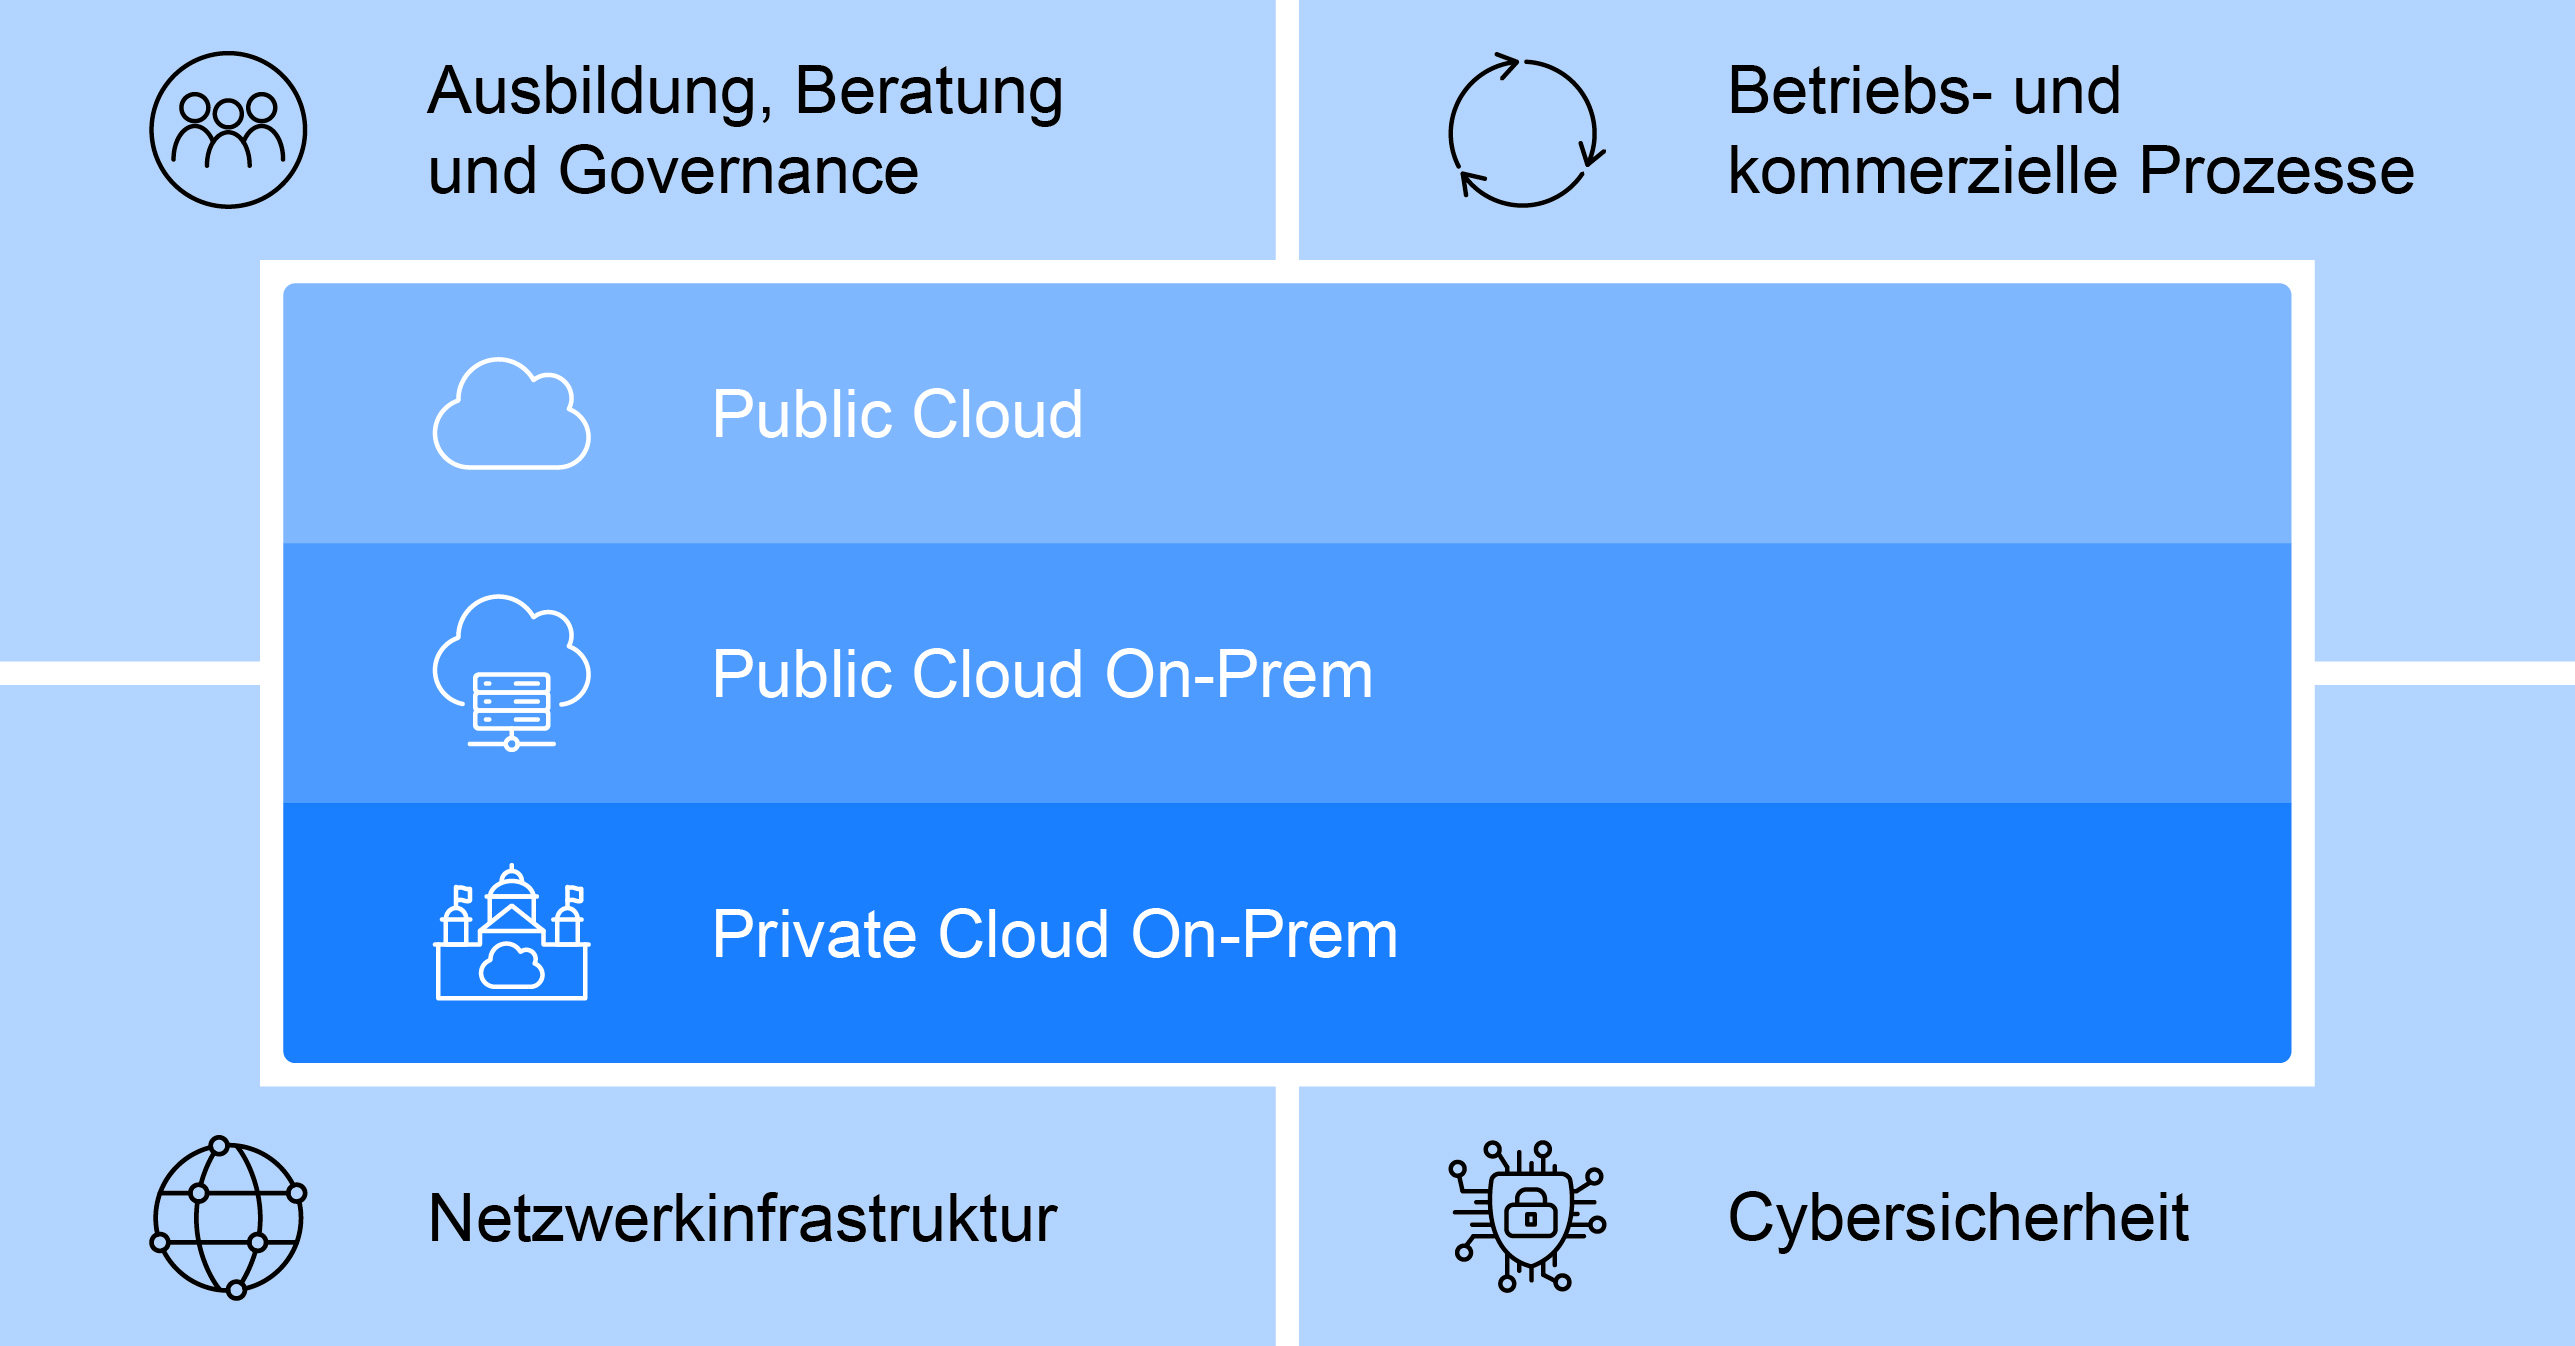
\includegraphics[width=\linewidth]{BIT_SGC_Overview.jpg}
    \end{center}
\caption{Das Vorhaben SGC im Überblick}
\label{fig:sgc_overview}
\end{figure}

Heute verteilt sich die Infrastruktur des Bundesamt für Informatik und Telekommunikation (nachfolgenden als BIT bezeichnet) vereinfacht dargestellt wie folgt:

\begin{itemize}
\item OnPremise/Private-Cloud Hosting Umgebung welches durch das BIT selbst betrieben wird
\item Public-Cloud Hosting Umgebung bei unterschiedlichen Cloud-Anbietern wie Microsoft Azure und Amazon AWS
\end{itemize}
